%! Author = adnansiddiquei
%! Date = 13/12/2023

\subsection{Q2 - Dataset B}\label{subsec:dataset-b}
    \begin{figure}
    \centering
    \begin{subfigure}{0.9\textwidth}
      \centering
      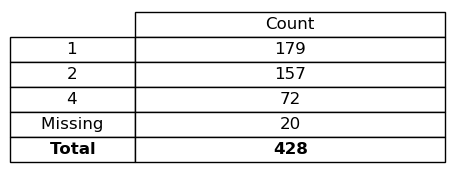
\includegraphics[width=.55\linewidth]{./figures/q2a}
      \caption{Raw \inlinecode{B_NoiseAdded.csv} dataset, before pre-processing. There are 428 observations with 20 missing
        labels and 20 duplicated observations (40 observations involved in the duplication).}
      \label{fig:q2a}
    \end{subfigure}%
    \hfill
    \begin{subfigure}{0.9\textwidth}
      \centering
      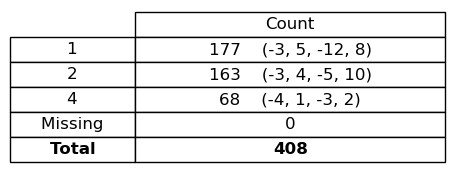
\includegraphics[width=0.55\linewidth]{./figures/q2b_q2d}
      \caption{\inlinecode{B_NoiseAdded.csv} after pre-processing, no missing labels or duplicated observations.
        The 4 numbers in the brackets indicate how the count in each classification changed due to, in order: 1 -
        count exiting class due to mislabelling; 2 - count entering class due to mislabelling; 3 - count exiting
        after dropping duplicates; 4 - count entering after imputation of missing labels.}
      \label{fig:q2bd}
    \end{subfigure}
    \caption{Summary of classifications for the \inlinecode{B_NoiseAdded.csv} dataset before and after pre-processing.}
    \label{fig:q2abd}
    \end{figure}

    Fig.\eqref{fig:q2a} shows the summary of classifications for the \inlinecode{B_NoiseAdded.csv} dataset.
    It was identified that the dataset contained 20 duplicated observations (a total of 40 observations involved in the
    duplication), and 10 of these duplicates contained different labels across the two duplicates.
    The correct assignment for this mislabelling was determined using multinomal logistic regression on the labelled data
    to predict the labels on the mislabelled data.
    Multinomal logistic regression was then used again to predict the labels for the 20 missing observations, and
    Fig.\eqref{fig:q2bd} shows the new summary of classifications.

    Generally, there are multiple ways to handle missing labels.
    One such way is model based imputation, which was used here.
    This is where an appropriate model is trained on the labelled data to predict the missing labels.
    Another option could be to ignore the data with the missing labels, if the sample size is sufficiently large enough.
    Model based imputation has the advantage of using all the data, however it can introduce bias if the model is not
    a great fit for the data.
    Ignoring the data is advantageous in that it won't create bias if the sample size is large enough.

    Missing at random (MAR) is when the likelihood that a label is missing is independent of the label itself, and
    missing not at random (MNAR) is when the likelihood of the label missing is in some way correlated with the value
    of the label.
    Looking at the 4th number in the brackets of Fig.\eqref{fig:q2bd}, which shows the number of observations that
    entered each classification after imputing the missing labels, it can be seen that no class had
    a significantly disproportionate number of observations enter it after imputation, indicating that the missing
    labels are likely MAR.
